\chapter{Concept and Modeling}
\label{ch:Concept} 

This chapter presents the core concepts, architectural models, and hardware components selected for the \acs{FPGA} Verification Platform Proof of Concept (PoC). The discussion begins with an examination of the Servo Drive Control Board Architecture, which defines the operational context and identifies the Design Under Test (DUT) modules. Subsequently, a Requirement Analysis is conducted to justify selecting the Enclustra Mercury XU5 and the DAC80508 as the primary verification hardware. The Block Design of the proposed \acs{PoC} is then introduced, illustrating the integration of these components into a closed-loop system for automated \acs{FPGA} module verification. The chapter concludes with a review of related work and case studies in \acs{FPGA} and Hardware-in-the-Loop (HIL) Verification, situating the platform's contribution within the broader research landscape.

\section{Servo Drive Control Board Architecture}
\label{sec:Concept:ServoDriveArch} 

Modern servo drives integrate advanced control electronics, optimized power efficiency, and comprehensive safety mechanisms within a compact, modular architecture. In industrial automation applications, such as those utilizing Schneider Electric’s PacDrive 3 platform, servo drives serve as the central components for synchronizing multi-axis control systems.

\begin{figure}[htbp]
	\centering
	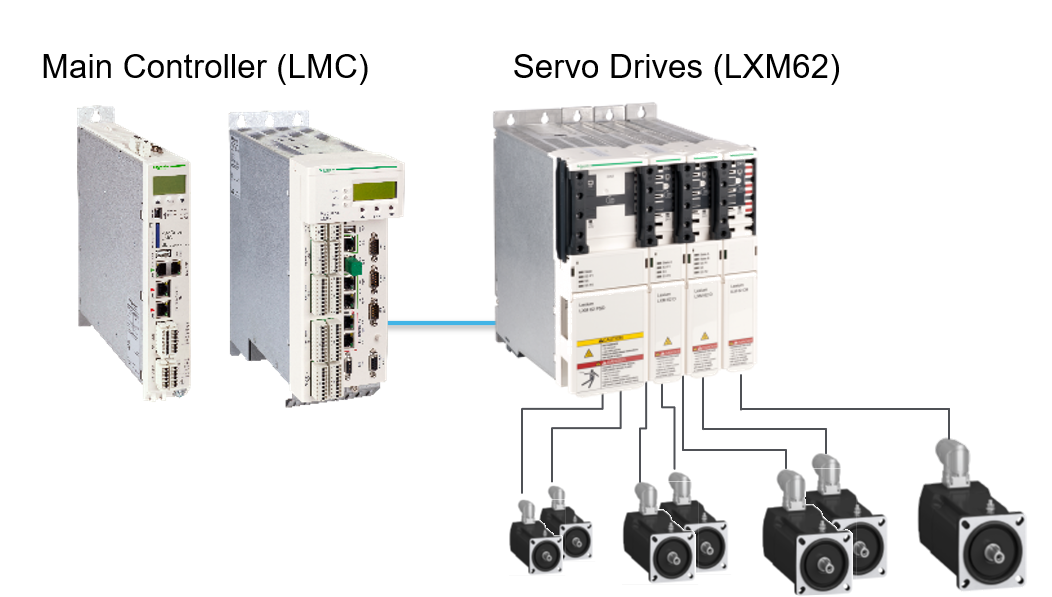
\includegraphics[width=1.00\textwidth]{gfx/diagrams/Pac_Drive_System.png}
	\caption{PacDrive 3 Platform. ServoDrive - System Architecture}
	\label{fig:concept:PacDrive3}
\end{figure}

The PacDrive 3 platform (figure \ref{fig:concept:PacDrive3}) comprises a central Logic Motion Controller (LMC) and multiple Lexium 62 servo drives, which are interconnected via a Sercos III real-time Ethernet network. The LMC manages motion planning, generates movement trajectories, and synchronizes all servo axes. Each Lexium 62 drive utilizes integrated electronics to regulate current and speed, continuously transmitting feedback to the LMC. This configuration facilitates system scalability, minimizes wiring requirements, and ensures precise real-time coordination among motion axes. Each servo drive has the following primary features \cite{PacDrive3HardwareGuide} \cite{SchneiderLexium62Catalog2022} :

\begin{enumerate}
	\item \textbf{Motion Control and Application Capabilities:} Lexium 62 drives employ advanced motion control and feedback systems to achieve rapid, smooth movements with minimal contouring error. This enables precise positioning and consistent performance in demanding servo applications. The drives are compatible with Schneider Electric’s Lexium SH3, MH3, and SHS stainless-steel servo motors, and can also interface with select third-party linear, torque, or asynchronous motors via encoder adapters, provided these motors comply with over voltage category III standards
	
	\item \textbf{Fast Connection Technology:} A key advantage of the Lexium 62 series is its Fast Connection design, which streamlines installation and integration. Each drive module features front-facing plug-in connections for the DC bus, 24 V power, and Sercos III communication, eliminating the need for complex back plane wiring. Through the Sercos motion bus, single-and double-axis drives integrate into the control network and communicate directly with the central Logic Motion Controller (LMC). The shared DC bus supplies up to 120 A of continuous current, enhancing energy efficiency and simplifying cabinet wiring for multi-axis systems.
	
	\item \textbf{Safety and Reliability Features:} Safety is integrated into both the hardware and communication systems. Standard drives incorporate a hardwired Safe Torque Off (STO) feature, certified to SIL 3/PLe, ensuring the motor remains torque-free during emergencies or faults. Advanced models provide additional safety functions beyond Sercos, including Safe Stop, Safe Operating Stop, and Safe Limited Speed, in compliance with IEC 61508 and EN ISO 13849-1. In multi-axis systems, Lexium 62 modules utilize a shared power supply and DC link, reducing cabinet space requirements and costs while maintaining safety.
	
	\item \textbf{Internal Functionalities and Drive Logic:} Beyond motion control, the drives incorporate multiple protective and adaptive features. These include torque limits that adjust with acceleration to prevent mechanical stress, detection of mechanical overloads, brake-release verification, and velocity control without an encoder when paired with \acs{BMP} motors. These intelligent features enhance reliability, safeguard components, and enable flexible operation even in the absence of complete encoder feedback.
\end{enumerate}

Figure \ref{fig:concept:ServoDrive_Arch_Seperation} illustrates the internal structure of a typical servo drive. The diagram distinguishes the Control Electronics, responsible for low-voltage and cold-side control, from the Power Electronics, which manage high-voltage and hot-side control.

 \begin{figure}[htbp]
 	\centering
 	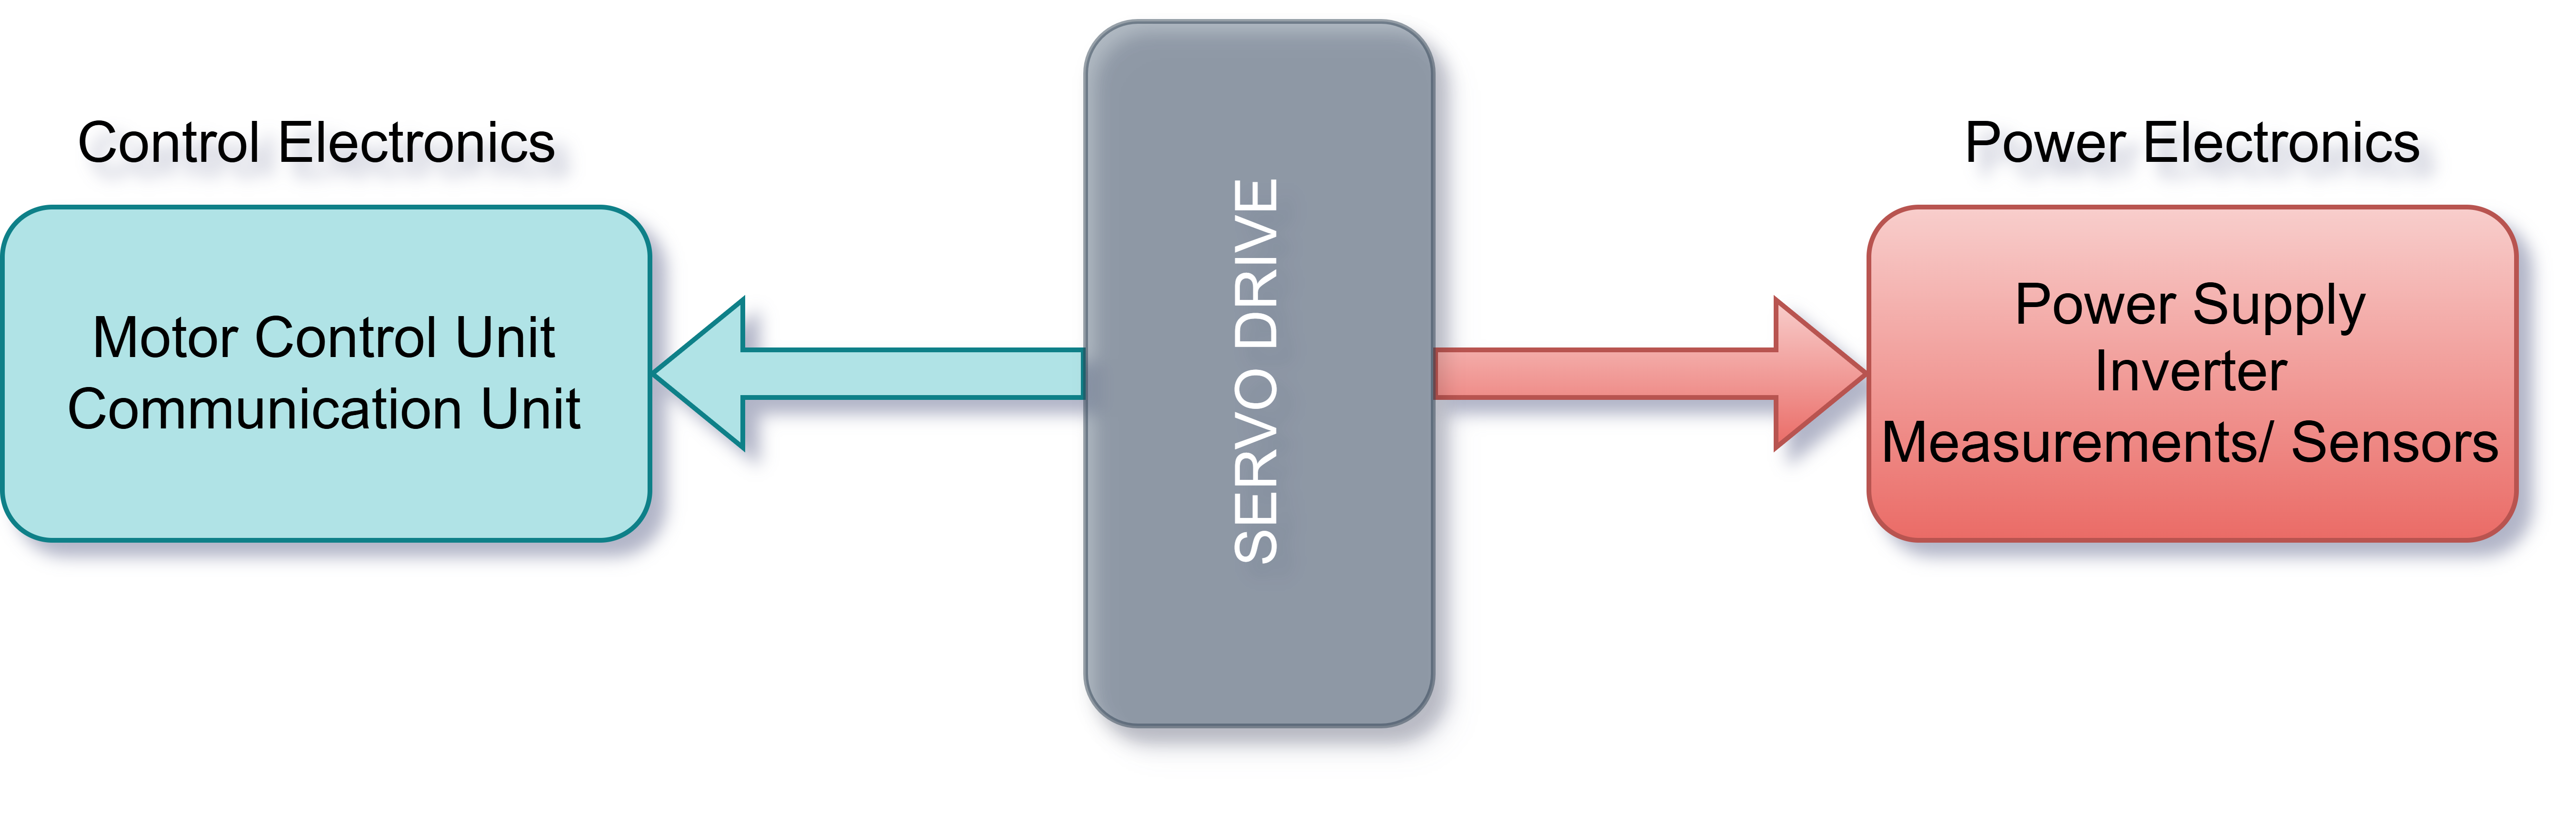
\includegraphics[width=0.80\textwidth]{gfx/diagrams/Servo_Drive_Logic_Division.png}
 	\caption{Architectural division of Servo Drive Control Board}
 	\label{fig:concept:ServoDrive_Arch_Seperation}
 \end{figure}

\begin{enumerate}
	\item \textbf{ Hot Side (Power / Motor Zone):}
	\begin{itemize}
		\item This section comprises the primary high-voltage and high-current components, including inverter bridges, DC bus elements, braking circuits, and motor windings.
		\item This delivers the necessary currents and voltages to the servo motor, facilitating precise regulation of torque, speed, and position.
	\end{itemize}
		\item \textbf{  Cold Side (Control / Logic Zone):}
	\begin{itemize}
		\item This section contains low-voltage electronic components, including controllers, isolated gate drivers, sensors, feedback circuits, logic circuits, and communication interfaces.
		\item The control logic and input/output circuits typically operate at supply voltages of 24 V or lower.
	\end{itemize}
\end{enumerate}

\begin{figure}[htbp]
	\centering
	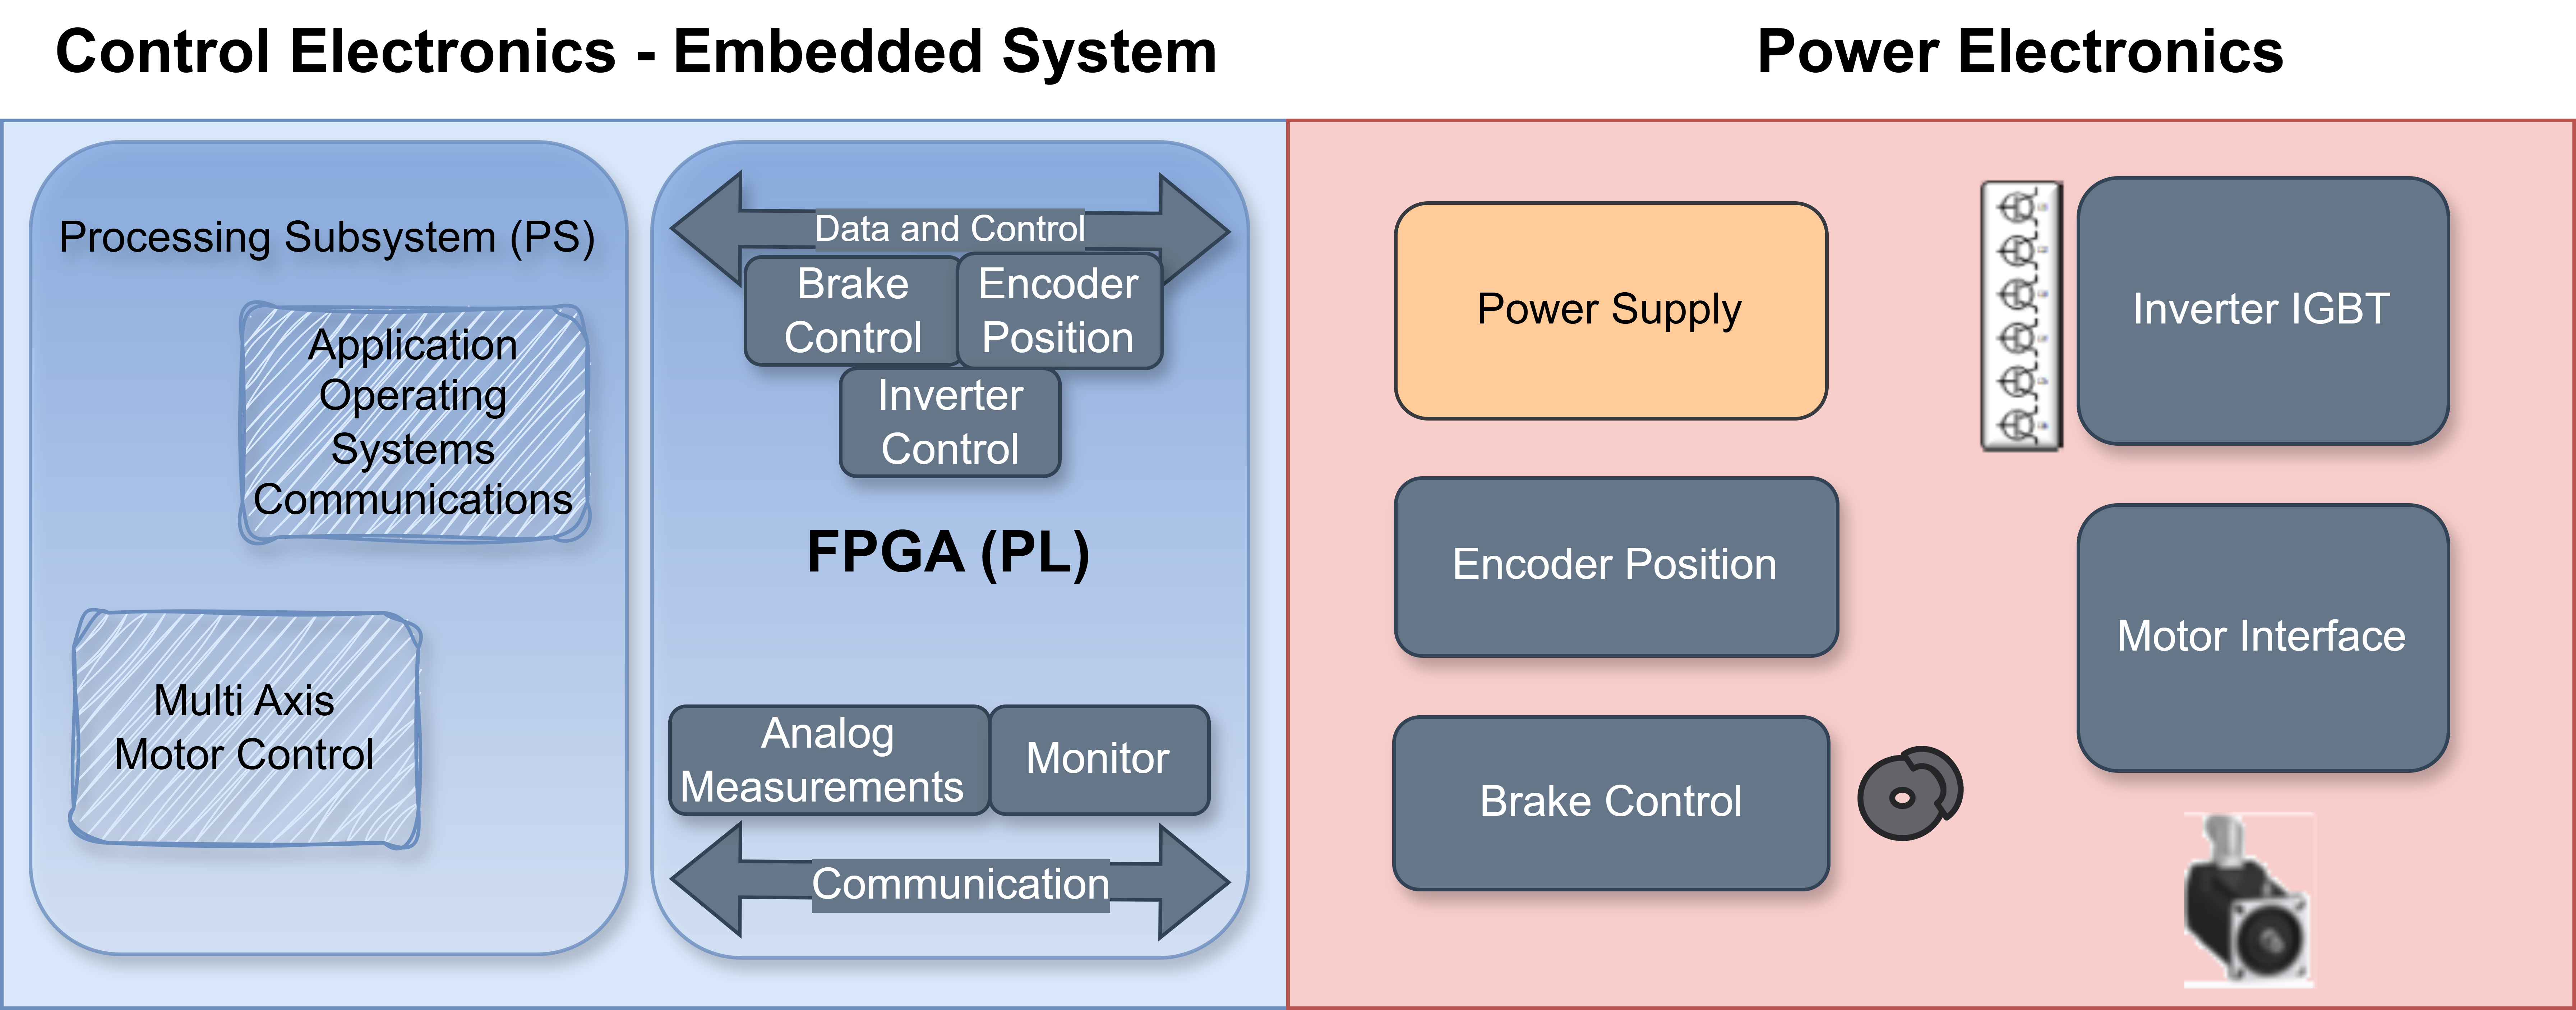
\includegraphics[width=0.80\textwidth, height=0.6\linewidth]{gfx/diagrams/Servo_Drive_Power_Control.png}
	\caption{Internal architecture of the servo drive showing separation between control (cold side) and power (hot side) electronics}
	\label{fig:concept:ServoDrive_Arch}
\end{figure}

%In a multi-servo Drive system, the Servo Drives are sharing a common DC Bus, and in a single servo drive system DC bus voltage is provided by a Power Supply which takes in AC mains and rectifies it, along with 24V low power supply. The Inverter (three phase IGBT bridge) consists of 6 IGBTs arranged in a bridge configuration, allowing the conversion of DC to AC. It operates by switching the IGBTs on and off in a specific sequence controlled by the PWM Signals to create the three-phase controlled AC output. The Servo drives do not apply the mains AC directly to the motor because the frequency, amplitude, and the phase of the mains supply cannot be controlled. The controlled converted 3 phase AC enables variable frequency, voltage, phase, amplitude and allows full-closed loop control over the Servo motors

In multi-axis servo drive systems, all drives utilize a shared high-voltage \acs{DC} bus as a central energy source. In contrast, single-axis configurations employ a dedicated power supply module that converts \acs{AC} mains into a stable, high-voltage \acs{DC} link and provides 24 V to the control electronics. Large capacitors on the \acs{DC} bus store energy, minimize voltage ripple, and absorb excess energy during braking or deceleration.

The inverter converts \acs{DC} power into controlled three-phase \acs{AC} using six insulated-gate bipolar transistors (IGBTs) arranged in a three-phase bridge configuration. Each \acs{IGBT} is switched on and off by high-frequency \acs{PWM} signals generated by the \acs{FPGA} or controller. These signals regulate the voltage supplied to each motor phase, producing current waveforms that closely approximate a sine wave with the desired amplitude, frequency, and phase. Unlike standard \acs{AC} mains, which cannot be dynamically adjusted, this controlled \acs{AC} enables variable speed operation, precise torque control, and comprehensive closed-loop regulation of motor position and speed. Continuous adjustment of the \acs{PWM} duty cycle based on sensor feedback ensures smooth motor operation, supports regenerative braking, and enables four-quadrant operation, thereby meeting the stringent requirements of modern industrial servo systems. 

An isolation barrier separates the high-voltage (\acs{DC} bus components) and logic zones (24V low voltage components) to prevent high voltage from reaching the logic side and to ensure galvanic separation. This barrier safeguards low-voltage logic circuits and enhances overall system safety. The cold-side control electronics, illustrated in figure \ref{fig:concept:ServoDrive_Arch}, and other low-voltage components typically incorporate a Zynq UltraScale+ \acs{MPSoC} \acs{FPGA}. This \acs{FPGA} is responsible for logic operations, computation, and real-time control. The \acs{PS} executes high-level functions, including motor and current control loops, communication, and diagnostics. The \acs{PL} performs time-critical operations, including brake control, inverter control, encoder position tracking, and safety monitoring. The \acs{FPGA} and processor utilize shared data interfaces to exchange control parameters and feedback in real time.

Within this architecture, the \acs{FPGA}-based control electronics form the core of the cold-side logic domain. These \acs{FPGA} modules represent the \acs{DUT} examined in this thesis. The following section provides a detailed description of their operation, including their inputs and outputs.

\section{Understanding the \acs{DUT}}
\label{sec:Concept:Understanding_DUTs}

The Figure \ref{fig:concept:ServoDrive_MPSoc_View} presents the block-level design of the \acs{MPSoC} \acs{FPGA} implemented on the control board. The ServoDrive system utilizes the Zynq UltraScale+ CG variant, which integrates a dual-core Arm Cortex-A53 application processor and a dual-core R5F real-time processor. In this diagram, blue blocks indicate \acs{FPGA} modules implemented and requiring comprehensive testing prior to the release of the control board. These modules perform essential functions to maintain the reliable operation of the ServoDrive system. Rigorous testing is necessary to ensure system stability, accurate signal processing, and compliance with real-time performance requirements.

\begin{figure}[htbp]
	\centering
	\includegraphics[width=0.80\textwidth]{gfx/diagrams/Servo_Drive_ControlBoard_PL_BlockDesign.png}
	\caption{Control Board \acs{MPSoC} View}
	\label{fig:concept:ServoDrive_MPSoc_View}
\end{figure}

This thesis examines \acs{FPGA} hardware modules designed for motor control and protection. In particular, it analyses the Current Sense \acs{SPI} module, which interfaces with the \acs{ADC} to acquire motor feedback (serving as the primary input to the servo drive's current control algorithm) and to monitor currents. The \acs{OVC}\_Detect module, which identifies over-current conditions, and the \acs{PWM} Control module, which generates pulse-width modulation signals for motor drive, are also evaluated. Focusing on these modules enables a comprehensive assessment of the system's critical control and safety features, as well as a systematic evaluation of the \acs{FPGA} implementation's overall functionality and performance.

\subsection{CurrentSense \acs{SPI} Path}
	\label{sec:Conecpt:UnderstandingDUTs:CurrentSensepath}
	
	 The figure \ref{fig:concept:CurrentSense_Block} depicts the Current Sense path on the control board. The board’s analog-to-digital converters (\acs{ADC}s) continuously acquire feedback signals from the motor phases. These analog signals, representing the instantaneous motor current, are converted to digital values and transmitted to the Current Sense \acs{SPI} module. The module processes these values and generates 12-bit digital outputs for subsequent control and monitoring. This signal path serves as the \acs{DUT} in this thesis and functions as a critical interface between the motor hardware and the digital control logic.

	 The primary objective of this work is to generate feedback signals that would typically originate from the motor hardware. This method enables testing and verification of the Current Sense \acs{SPI} module in a controlled environment. By producing both static and dynamic test signals, the module’s response to various conditions, such as constant currents, abrupt changes, and variations in motor load, can be thoroughly evaluated. This methodology enables a comprehensive assessment of the accuracy, resolution, and timing of the Current Sense \acs{SPI} outputs, ensuring the module meets all specified requirements before integration with the actual motor system.


		\begin{figure}[H]
			\centering
			% Scaling kept at 70% and node distance at 3.5cm to ensure the current width is intact
			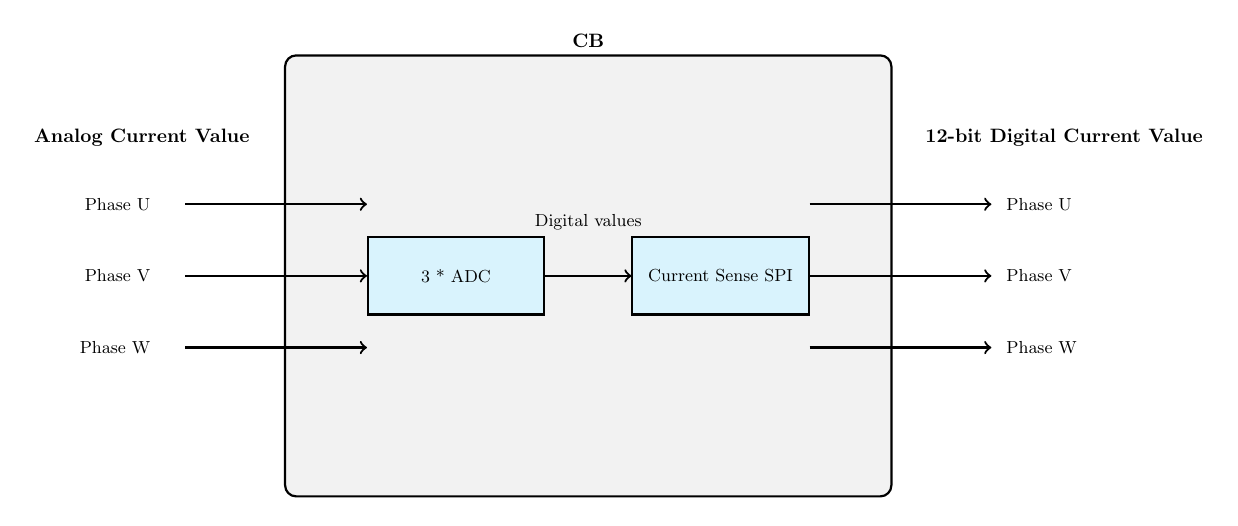
\begin{tikzpicture}[node distance=3.5cm, auto, thick, font=\sffamily, scale=0.7, transform shape]
				
				% Define styles using \tikzset (modern practice)
				\tikzset{
					mainbox/.style = {
						draw, fill=gray!10, rounded corners,
						minimum width=11cm, 
						% Minimum height set to 8.0cm
						minimum height=8.0cm, 
						label={[font=\bfseries]above:CB} 
					},
					subblock/.style = {
						draw, fill=cyan!15, 
						minimum width=3.2cm,
						minimum height=1.4cm, 
						align=center, 
						font=\small
					},
					arrow/.style = {->, thick}
				}
				
				% Main Control Board box
				\node[mainbox] (cb) {};
				
				% Internal sub-blocks
				\node[subblock] (adc) at ([xshift=-2.4cm]cb.center) {3 * \acs{ADC}};
				\node[subblock] (spi) at ([xshift=2.4cm]cb.center) {Current Sense \acs{SPI}};
				
				% Connection between ADC and SPI
				\draw[arrow] (adc.east) -- (spi.west)
				% Gap for text kept at 20pt
				node[midway, above=20pt, font=\small, align=center] {Digital values};
				
				% ==== INPUT ARROWS (3 lines, vertically spaced, labels outside) ====
				
				% Title: Moved UP and slightly RIGHT
				\node[left=2.0cm, font=\bfseries] at ([yshift=2.5cm]adc.west) {Analog Current Value};
				
				% Updated labels for individual phase arrows (Phase U, V, W)
				\foreach \y/\label in {1.3/Phase U, 0/Phase V, -1.3/Phase W}{
					% Arrows start farther left (xshift=-5.5cm) to accommodate the new bold label
					\draw[arrow] ([xshift=-3.3cm,yshift=\y cm]adc.west) -- ([yshift=\y cm]adc.west);
					% REDUCED horizontal gap: changed left=1.5cm to left=0.5cm
					\node[left=0.5cm, font=\small] at ([xshift=-3.3cm,yshift=\y cm]adc.west) {\label};
				}
				
				% ==== OUTPUT ARROWS (3 lines, vertically spaced, labels outside) ====
				
					% Title: Moved UP and slightly RIGHT
				\node[right=10.0cm, font=\bfseries] at ([yshift=2.5cm]adc.west) {12-bit Digital Current Value};
				
				\foreach \y/\label in {1.3/Phase U, 0/Phase V, -1.3/Phase W}{
					\draw[arrow] ([yshift=\y cm]spi.east) -- ([xshift=3.3cm,yshift=\y cm]spi.east);
					\node[right=4pt, font=\small] at ([xshift=3.3cm,yshift=\y cm]spi.east) {\label};
				}
				
			\end{tikzpicture}
			\caption{Simplified block representation of the three-phase current-sensing chain within the control board}
			\label{fig:concept:CurrentSense_Block}
		\end{figure}

\subsection{\acs{OVC} Detect}
\label{sec:Conecpt:UnderstandingDUTs:OVC_Detect}
	
	The \acs{OVC} Detect module identifies overcurrent or short-circuit conditions on any of the three motor phases (U, V, or W) and subsequently disables the \acs{PWM} outputs to protect the system. Detection thresholds are configurable via the \acs{AXI} interface, allowing adjustment of both the lower limit for overcurrent and the upper limit for short-circuit detection. The \acs{OVC} Detect module operates in conjunction with the Current Sense \acs{SPI} module (refer figure \ref{fig:concept:OVCD_Block}) and is triggered whenever a new current measurement becomes available. It continuously compares the measured current values from all three phases to the configured threshold limits. Based on these comparisons, the module issues two signals: \acs{OVC} status, which indicates the current fault condition, and \acs{OVC} event, which serves as a fault notification.
	
	Within the module, a finite state machine controls two primary error states.
\begin{itemize}
\item \textbf{Overcurrent:} The system transitions to this state if an overcurrent is detected in any of the three phases (U, V, or W). If the overcurrent persists for approximately 10 microseconds, the state advances to a short-circuit condition.	
\item \textbf{Short-Circuit:} In this state, the module sets the ovc\_event output signal to logic ‘1’, indicating a severe fault that requires immediate shutdown of the \acs{PWM}.
\end{itemize}

	
	\begin{figure}[H]
	\centering
	% Scaling kept at 70% and node distance at 3.5cm to ensure the current width is intact
	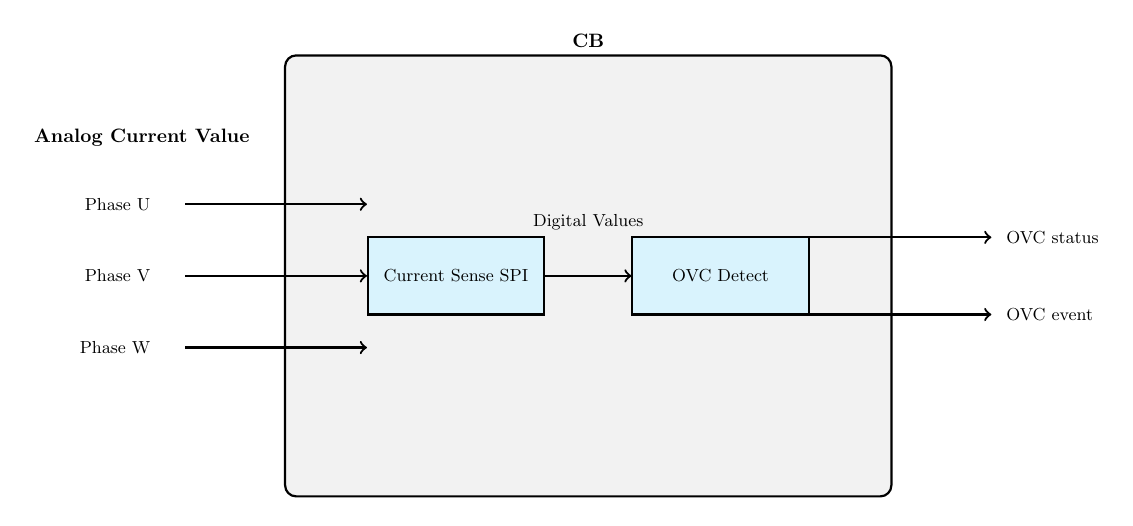
\begin{tikzpicture}[node distance=3.5cm, auto, thick, font=\sffamily, scale=0.7, transform shape]
				
			% Define styles using \tikzset (modern practice)
			\tikzset{
				mainbox/.style = {
					draw, fill=gray!10, rounded corners,
					minimum width=11cm, 
					% Minimum height set to 8.0cm
					minimum height=8.0cm, 
					label={[font=\bfseries]above:CB} 
				},
				subblock/.style = {
					draw, fill=cyan!15, 
					minimum width=3.2cm,
					minimum height=1.4cm, 
					align=center, 
					font=\small
				},
				arrow/.style = {->, thick}
			}
			
			% Main Control Board box
			\node[mainbox] (cb) {};
				
				% Internal sub-blocks: First block is Current Sense SPI, second is OVC Detect
				\node[subblock] (spi) at ([xshift=-2.4cm]cb.center) {Current Sense \acs{SPI}};
				\node[subblock] (ovcd) at ([xshift=2.4cm]cb.center) {\acs{OVC} Detect};
				
				% Connection between SPI and OVC Detect
				\draw[arrow] (spi.east) -- (ovcd.west)
				% Label for the connection
				node[midway, above=20pt, font=\small, align=center] {Digital Values};
				
				% ==== INPUT ARROWS (3 lines, vertically spaced, labels outside) INTO Current Sense SPI ====
				
				% Title: Input title (representing the output of the previous stage)
				\node[left=2.0cm, font=\bfseries] at ([yshift=2.5cm]spi.west) {Analog Current Value};
				
				% Updated labels for individual phase arrows (Phase U, V, W)
				\foreach \y/\label in {1.3/Phase U, 0/Phase V, -1.3/Phase W}{
					% Arrows start farther left
					\draw[arrow] ([xshift=-3.3cm,yshift=\y cm]spi.west) -- ([yshift=\y cm]spi.west);
					% Label placement
					\node[left=0.5cm, font=\small] at ([xshift=-3.3cm,yshift=\y cm]spi.west) {\label};
				}
				
				% ==== OUTPUT ARROWS (2 lines) FROM OVC Detect ====
				
				% Output 1: OVC status (Higher position)
				\draw[arrow] ([yshift=0.7cm]ovcd.east) -- ([xshift=3.3cm,yshift=0.7cm]ovcd.east);
				\node[right=4pt, font=\small] at ([xshift=3.3cm,yshift=0.7cm]ovcd.east) {\acs{OVC} status};
				
				% Output 2: OVC event (Lower position)
				\draw[arrow] ([yshift=-0.7cm]ovcd.east) -- ([xshift=3.3cm,yshift=-0.7cm]ovcd.east);
				\node[right=4pt, font=\small] at ([xshift=3.3cm,yshift=-0.7cm]ovcd.east) {\acs{OVC} event};
				
				% Removed the '12-bit Digital Current Value' output title
				
			\end{tikzpicture}
			\caption{Simplified block representation of the Over-Current Detect path within the control board}
			\label{fig:concept:OVCD_Block}
		\end{figure}
	
	
\subsection{\acs{PWM} Control}
\label{sec:Conecpt:UnderstandingDUTs:PWM_Control}
	
	The \acs{PWM}\_IP module (figure \ref{fig:concept:PWM_Block}) generates \acs{PWM} signals to drive the motor phases. It receives the desired frequency and duty cycle as inputs and produces corresponding \acs{PWM} waveforms. The module supports three selectable switching frequencies: 16 kHz, 8 kHz, or 4 kHz, allowing adaptation to specific motor control requirements. It provides six \acs{PWM} outputs, corresponding to the high-side and low-side signals for the three motor phases (U, V, and W). Although all six signals operate at the same switching frequency, each can be assigned an independent duty cycle, enabling flexible control and modulation for various operational scenarios.
	
	In the current system, the \acs{PWM}\_IP module drives the motor hardware. The \acs{PWM} signals are transmitted to the motor inverter stage, which generates phase currents in the motor windings. The control board’s \acs{ADC}s measure these phase currents, and the Current Sense \acs{SPI} module processes the data for feedback and monitoring. Due to this interdependent configuration, several \acs{FPGA} modules and hardware components rely on one another, necessitating the involvement of multiple modules during testing.
	
	\begin{figure}[H]
		\centering
		% Scaling kept at 70% and node distance at 3.5cm to ensure the current width is intact
		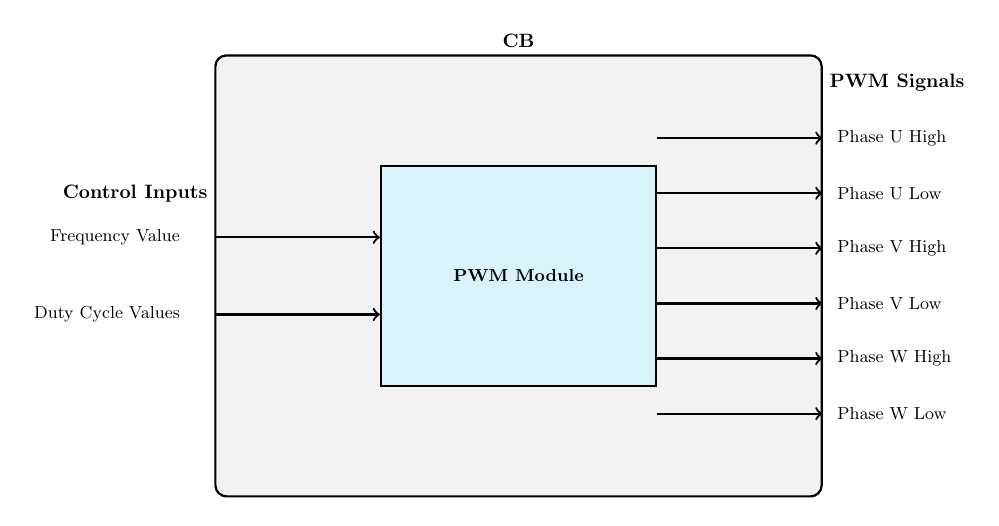
\begin{tikzpicture}[node distance=3.5cm, auto, thick, font=\sffamily, scale=0.7, transform shape]
			
			% Define styles using \tikzset (modern practice)
			\tikzset{
				mainbox/.style = {
					draw, fill=gray!10, rounded corners,
					minimum width=11cm,
					% Corrected the key name by removing any potential space
					minimum height=8.0cm,
					label={[font=\bfseries]above:CB}
				},
				subblock/.style = {
					draw, fill=cyan!15,
					minimum width=5.0cm, % Widened to accommodate text
					minimum height=4.0cm, % Increased height to accommodate inputs/outputs
					align=center,
					font=\small
				},
				arrow/.style = {->, thick}
			}
			
			% Main Control Board box
			\node[mainbox] (cb) {};
			
			% Internal sub-block: PWM is centered
			% NAME CHANGED HERE: PWM IP Module -> PWM Module
			\node[subblock] (pwm) at (cb.center) {\textbf{\acs{PWM} Module}};
			
			% ==== INPUT ARROWS (2 lines, vertically spaced) INTO PWM ====
			
			% Input 1: Frequency
			\node[left=3.0cm, font=\bfseries] at ([yshift=1.5cm]pwm.west) {Control Inputs};
			\draw[arrow] ([xshift=-3.0cm,yshift=0.7cm]pwm.west) -- ([yshift=0.7cm]pwm.west);
			\node[left=0.5cm, font=\small] at ([xshift=-3.0cm,yshift=0.7cm]pwm.west) {Frequency Value};
			
			% Input 2: Duty Cycle
			\draw[arrow] ([xshift=-3.0cm,yshift=-0.7cm]pwm.west) -- ([yshift=-0.7cm]pwm.west);
			\node[left=0.5cm, font=\small] at ([xshift=-3.0cm,yshift=-0.7cm]pwm.west) {Duty Cycle Values};
			
			% ==== OUTPUT ARROWS (6 lines, vertically spaced) FROM PWM ====
			
			% Title for outputs
			\node[right=3.0cm, font=\bfseries] at ([yshift=3.5cm]pwm.east) {PWM Signals};
			
			\foreach \y/\label in {2.5/Phase U High, 1.5/Phase U Low, 0.5/Phase V High, -0.5/Phase V Low, -1.5/Phase W High, -2.5/Phase W Low}{
				% Arrows start at the right of the block
				\draw[arrow] ([yshift=\y cm]pwm.east) -- ([xshift=3.0cm,yshift=\y cm]pwm.east);
				% Label placement
				\node[right=4pt, font=\small, align=left] at ([xshift=3.0cm,yshift=\y cm]pwm.east) {\label};
			}
			
		\end{tikzpicture}
		\caption{Simplified block representation of the \acs{PWM} Generation Module within the control board}
		\label{fig:concept:PWM_Block}
	\end{figure}
	
	The interdependency among modules during verification complicates the isolation and testing of individual module functionality. Therefore, a dedicated \acs{FPGA} Verification Platform is required to enable independent verification of \acs{FPGA} modules and address the limitations identified in the problem statement [\ref{sec:intro:ProblemStatement}]. The subsequent section presents the Requirement Analysis of the \acs{PoC} for the proposed \acs{FPGA} Verification Platform.

\section{Requirement Analysis}
\label{sec:Concept:RequirementAnalysis}

The primary objective of the proposed verification platform is to emulate the necessary input stimuli for the specific \acs{DUT} (\acs{FPGA} modules), implemented on the control board, and to capture and analyze the corresponding feedback to determine whether each \acs{DUT} operates as intended. To accomplish this, the verification platform must be implemented on an \acs{FPGA} or \acs{SoC} from the same family as the one used on the control board. This approach ensures architectural, timing, and interface compatibility, thereby facilitating accurate emulation and reliable verification outcomes. Several factors support selecting an \acs{FPGA} over a microcontroller for this application:
\begin{itemize}
	\item \textbf{Parallel Verification:} The system should support simultaneous execution of multiple verification tasks. This parallelism substantially reduces overall verification time and serves as a primary motivation for developing a dedicated platform.
	\item \textbf{Clock Flexibility:} The control board may operate at different clock frequencies across development stages, the verification platform must support multiple clock domains and remain compatible with all versions and configurations of the control board.
	\item \textbf{Multiple DUTs:} The control board integrates several \acs{FPGA} modules that require functional verification. As additional features or modules are incorporated into the control board, the verification platform must adapt to emulate new input conditions and analyze the outputs of these expanded modules.
	\item \textbf{Extensibility:} The platform should be designed for scalability in both hardware architecture and verification logic, enabling straightforward integration of future test scenarios and additional \acs{FPGA} components.
\end{itemize}

\subsection{Enclustra Mercury XU5 + PE1 Evaluation board}

The \acs{FPGA} Verification Platform \acs{PoC} employs the Enclustra Mercury XU5 SoM (figure \ref{fig:concept:Mercury_XU5}) mounted on the Mercury+ PE1 Base Board (figure  \ref{fig:concept:Mercury_PE1}). This combination constitutes a high-performance platform built upon the heterogeneous architecture of the AMD Xilinx Zynq UltraScale+ \acs{MPSoC} \cite{Enclustra_XU5_Manual_2019}.

\begin{figure}[htbp]
	\centering
	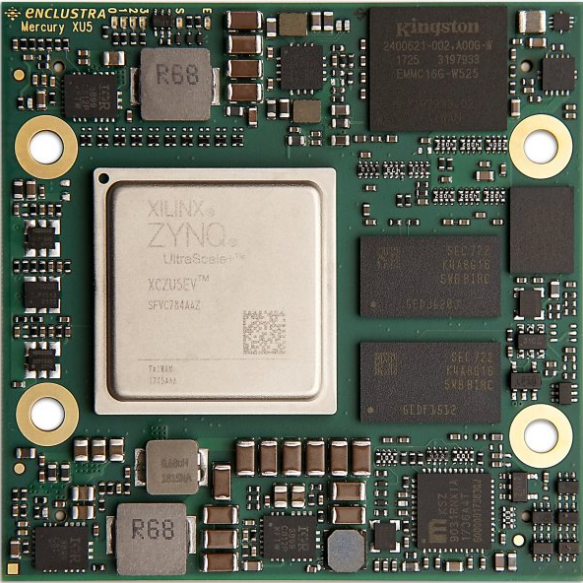
\includegraphics[width=0.45\textwidth]{gfx/diagrams/Mercury_XU5_SOC.png}
	\caption{Mercury XU5 SoM Top View Module \cite{Enclustra_XU5_Manual_2019}}
	\label{fig:concept:Mercury_XU5}
\end{figure}

%\vspace{-0.5\baselineskip}
\textbf{Mercury XU5 \acs{SoC} Module: Processing Core} \newline
The Mercury XU5 SoM serves as the primary processing core and is based on the AMD Zynq UltraScale+ \acs{MPSoC} \cite{Enclustra_XU5_Manual_2019}. This module provides a fully embedded processing system comprising the following key components:
\begin{itemize}
	\item \textbf{Processing System:} The processing system integrates multiple ARM cores, including a quad-core Cortex-A53 for application management and a dual-core Cortex-R5 for real-time control \cite{Enclustra_XU5_Manual_2019}.
	\item \textbf{Programmable logic:} The \acs{PL} fabric provides up to 256,000 \acs{LUT} equivalents, which hosts the core \acs{FPGA} modules \cite{Enclustra_XU5_Manual_2019}.
	\item \textbf{Memory Architecture:} The module includes two independent \acs{DDR4 SDRAM} channels with ECC support for the processing system and supports high-bandwidth data transfer \cite{Enclustra_XU5_Manual_2019}. 
\end{itemize}	

\begin{figure}[H]
	\centering
	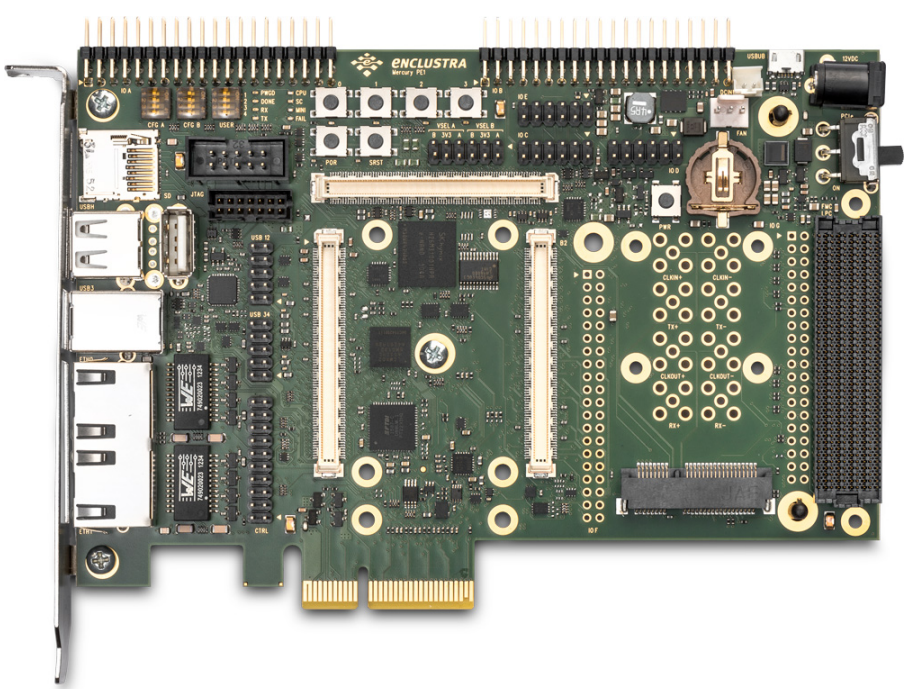
\includegraphics[width=0.70\textwidth]{gfx/diagrams/Mercury_PE1.png}
	\caption{Mercury PE1 Board Top View \cite{Enclustra_PE1_Manual_2020}}
	\label{fig:concept:Mercury_PE1}
\end{figure}

\textbf{Mercury+ PE1 Base Board: Interface and I/O} \newline
The Mercury+ PE1 Base Board functions as a versatile carrier, providing the necessary physical interfaces and I/O connections for the SoM. The primary features of the PE1 Base Board supporting the \acs{PoC} include:
\begin{itemize}
	\item \textbf{FMC Connectors:} The board accommodates up to two FMC Low Pin Count (LPC) connectors, enabling expansion for custom data acquisition or specialized \acs{DAC} components \cite{Enclustra_PE1_Manual_2020}.
	\item \textbf{Communication:}  The board provides \acs{PCIe} Gen2$\times$4, USB 3.0, and multiple USB 2.0 interfaces, which are essential for host PC communication and debugging \cite{Enclustra_PE1_Manual_2020}.
	\item \textbf{Flexibility:} The architecture supports use as either a standalone board or a \acs{PCIe} card, which is advantageous during the rapid prototyping phase \cite{Enclustra_PE1_Manual_2020}.
\end{itemize}
	
\subsection{DAC80508 Evaluation Board}

There is also a need for a \acs{DAC} to convert the digital sine wave generated by the Verification Platform \acs{FPGA} into an analog signal. Because the analog current values typically produced by physical motors are now emulated, this conversion is essential for verifying the CurrentSense \acs{SPI} and \acs{OVC} modules, as described in Section \ref{sec:Concept:Understanding_DUTs}.
\begin{figure}[t]
	\centering
	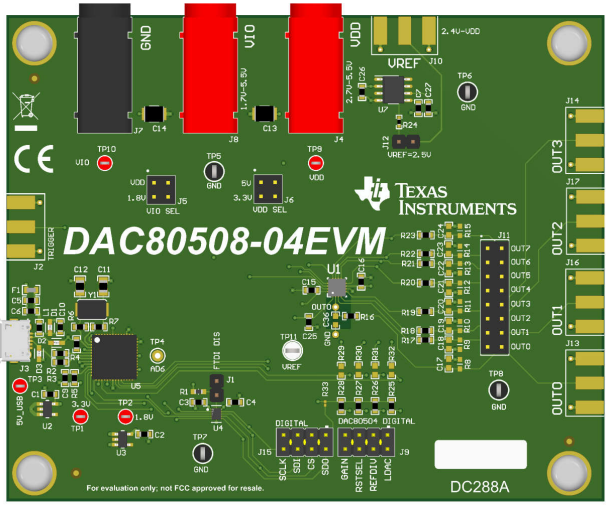
\includegraphics[width=0.60\textwidth]{gfx/diagrams/DAC80508.png}
	\caption{DAC80508-04EVM Evaluation board Top View \cite{TI_DAC80508_EVM_Guide}}
	\label{fig:concept:DAC80508}
\end{figure}
The DAC80508-04EVM evaluation board (figure \ref{fig:concept:DAC80508}) facilitates the interfacing and evaluation of the DAC80508, a high-resolution, multi-channel \acs{DAC}. The DAC80508 is part of the DACx0508 family of pin-compatible devices and is distinguished by its low power consumption, eight-channel architecture, and buffered voltage output \cite{TI_DAC80508}.

\begin{enumerate}
	\item \textbf{Key Integrated Features \cite{TI_DAC80508}}
	\begin{itemize}
		\item Resolution : The DAC80508 provides 16-bit resolution, resulting in highly granular analog signals and reduced quantization error and distortions, which is essential for smoother waveform reproduction.
		\item Internal Reference : The device integrates a 2.5 V precision internal reference, which typically eliminates the requirement for an external reference. This internal reference is accessible at the REF pin.
		\item Operating Range : It operates reliably across a wide temperature range from –40°C to 125°C.
		\item Output Configuration : Each of the eight output channels (OUT0 to OUT7) supports individual gain configuration. User-selectable gain settings (x2, x1, or ½) allow flexible output configuration. With the internal 2.5 V reference, these settings provide full-scale output voltages of 1.25 V, 2.5 V, or 5 V.
	\end{itemize}
		
	\item  \textbf{Digital Interface and Communication \cite{TI_DAC80508}}
	\begin{itemize}
		\item Serial Interface: Communication with the DAC80508 is accomplished via a \acs{SPI} compatible interface, supporting clock rates up to 50 MHz.
		\item Supply Flexibility: The digital interface (VIO pin) operates from 1.7 V to 5.5 V, enabling compatibility with a broad range of microprocessors and microcontrollers.
		\item Data Integrity: The device supports an optional \acs{CRC} error check, which improves robustness in noisy environments by verifying \acs{SPI} data integrity.
		\item Multi-Device Operation: The device supports daisy chain operation, allowing multiple DACx0508 devices to be connected together to minimize the number of required serial interface lines.		
	\end{itemize}
\end{enumerate}

Several registers are available; however, the configuration, gain, status, and DACx registers are most pertinent to the objectives of this thesis.

\begin{enumerate}
	\item \textbf{CONFIG Register} \newline
	\textbf{Address: 0x03 \textbar\space Default Value: 0x0000 \textbar\space	Access: Read/Write} \newline
	The CONFIG register (refer table \ref{table:Concept_and_Modeling:CONFIG_REG}) governs essential device operations, such as alarm triggering mechanisms, serial data output configuration, and the power-down status of \acs{DAC} channels.

	\begin{table}[htbp]
	\centering
	\caption{\textbf{CONFIG Register (Address = 0x03, Reset = 0x0000) \cite{TI_DAC80508}}}
	\label{table:Concept_and_Modeling:CONFIG_REG}
	\setlength{\fboxsep}{0pt}
	\fbox{%
		\begin{tabularx}{\textwidth}{c c c c X}
			\toprule
			\textbf{Bits} & \textbf{Field} & \textbf{Access} & \textbf{Reset} & \textbf{Function} \\
			\midrule
			15--14 & Reserved & -- & 00 &  Internal factory use only. \\
			\midrule
			13 & ALM\_SEL & R/W & 0 & This setting determines the function of the ALARM signal: a value of 0 indicates a \acs{CRC} error, while a value of 1 indicates a reference-voltage alarm. \\
			\midrule
			12 & ALM\_EN & R/W & 0 & Configures the SDO/ALARM pin to function either as a standard serial data output (0) or as an active-low, open-drain alarm output (1), requiring a 10 kΩ pull-up resistor. When enabled, the FSDO and DSDO signals are disregarded.\\
			\midrule
			11 & \acs{CRC}\_EN & R/W & 0 &A Value of 1 enables \acs{CRC} checking of serial data, whereas a value of 0 disables this feature.\\
			\midrule
			10 & FSDO & R/W & 0 & Modifies the timing of SDO updates. When enabled, data is presented half a clock cycle earlier, specifically on the falling edge of SCLK.\\
			\midrule
			9 & DSDO & R/W & 0 & When enabled, the SDO line remains in high-impedance mode continuously. \\
			\midrule
			8 & REF\_PWDWN & R/W & 0 & A value of 1 powers down the internal reference.\\
			\midrule
			7--0 & DACx\_PWDWN & R/W & 0 & Each bit corresponds to a \acs{DAC} channel (DAC0-DAC7). Setting a bit to 1 powers down the associated channel and connects its output to ground via an internal 1 kΩ resistor.\\
			\bottomrule
		\end{tabularx}%
	}
	\end{table}
	
	\item \textbf{GAIN Register} \newline
	\textbf{Address: 0x04 \textbar\space Access: Read/Write} \newline
	This register (see table \ref{table:Concept_and_Modeling:GAIN_Reg}) controls output gain and reference division. The default configuration depends on device type:  DACx0508Z models use a gain of 1, whereas DACx0508M models use a gain of 2.
	
	\begin{table}[htbp]
		\centering
		\caption{\textbf{GAIN Register (Address = 0x04) \cite{TI_DAC80508}}}
		\label{table:Concept_and_Modeling:GAIN_Reg}
		\setlength{\fboxsep}{0pt}
		\fbox{%
			\begin{tabularx}{\textwidth}{c c c c X}
				\toprule
				\textbf{Bits} & \textbf{Field} & \textbf{Access} & \textbf{Default} & \textbf{Description} \\
				\midrule
				15--11 & Reserved & -- & 0 & Internal factory use only. \\
				10 & CLR\_4TO7\_MSK & R/W & 0 & (DACx0508C only) When 0, DAC4--7 respond to CLR pin; when 1, unaffected. \\
				9 & CLR\_0TO3\_MSK & R/W & 0 & (DACx0508C only) When 0, DAC0--3 respond to CLR pin; when 1, unaffected. \\
				8 & REFDIV\_EN & R/W & 0/1 & Enables reference divider. When 1, reference voltage is halved. \\
				7--0 & BUFFx\_GAIN & R/W & 0/1 & Per-channel output buffer gain. 0: Gain = 1; 1: Gain = 2. \\
				\bottomrule
			\end{tabularx}
			}
	\end{table}
	
	\item \textbf{STATUS Register} \newline
	\textbf{Address: 0x07 \textbar\space Default Value: 0x0000 \textbar\space Access: Read-only} \newline
	This register indicates the present status of the reference voltage.
	
	\begin{table}[htbp]
		\centering
		\caption{\textbf{STATUS Register (Address = 0x07, Reset = 0x0000)} \cite{TI_DAC80508}}
		\label{table:Concept_and_Modeling:STATUS_Reg}
		\setlength{\fboxsep}{0pt}
		\fbox{%
		\begin{tabularx}{\textwidth}{c c c c X}
			\toprule
			\textbf{Bits} & \textbf{Field} & \textbf{Access} & \textbf{Default} & \textbf{Description} \\
			\midrule
			15--1 & Reserved & -- & 0 & Internal factory use only. \\
			0 & REF\_ALM & R & 0 & Indicates a reference alarm if V\textsubscript{REF}/DIV drops below the minimum threshold. \\
			\bottomrule
		\end{tabularx}
		}
	\end{table}
	
	\item \textbf{\acs{DAC} Channel Data Registers(DAC0- DAC7)} \newline
	\textbf{Address: 0x08 - 0x0F \textbar\space Access: Read/Write} \newline
	Each of the eight registers(Table \ref{table:Concept_and_Modeling:DAC_Reg})  contains a digital value that determines the analog output of a \acs{DAC} channel.

	\begin{table}[htbp]
		\centering
		\caption{\textbf{DACx Registers (Addresses = 0x08 to 0x0F) \cite{TI_DAC80508}}}
		\label{table:Concept_and_Modeling:DAC_Reg}
		\setlength{\fboxsep}{0pt}
		\fbox{%
		\begin{tabularx}{\textwidth}{c c c c X}
			\toprule
			\textbf{Bits} & \textbf{Field} & \textbf{Access} & \textbf{Default} & \textbf{Description} \\
			\midrule
			15--0 & DACx\_DATA & R/W & 0x0000 / 0x8000 & Holds the digital input code for each \acs{DAC} channel (MSB-aligned straight binary). Default is zero for Z devices and midscale for M devices. \\
			\bottomrule
		\end{tabularx}
		}
	\end{table}
\end{enumerate}

Owing to its high performance, compact package, and broad temperature range, the DACx0508 is suitable for applications such as optical networking, wireless infrastructure, industrial automation, and data acquisition systems \cite{TI_DAC80508_EVM_Guide}. The DAC80508-04EVM serves as a robust platform for evaluating an eight-channel, 16-bit-precision voltage-output \acs{DAC}, low-drift internal reference, selectable output gains, and advanced digital capabilities, including \acs{ACS} error checking and per-channel power-down. The following section presents a detailed explanation of the Block Design for the \acs{FPGA} Verification Platform \acs{PoC}.
	
\subsection{Block Design of the proposed \acs{FPGA} Verification Platform (Proof of concept)}

The Proof of Concept setup includes the Servo Drive Control Board, Enclustra Mercury XU5 Som, the PE1 board, and the DAC80508 Evaluation Board (refer figure \ref{fig:concept:PoC}). The Zynq UltraScale+ \acs{MPSoC} on the Mercury XU5 generates static and dynamic input signals, which trigger the \acs{DAC} to produce the analog signals required for CurrentSense \acs{SPI} verification as mentioned in section \ref{sec:Concept:Understanding_DUTs}. These analog signals serve as simulated motor current feedback and are connected to the \acs{ADC}s on the Hot Side of the control board. This configuration replaces the physical motor with a digitally controlled analog system, enabling closed-loop testing of the sensing and protection modules.

During each verification test, the \acs{SoC} transmits specific commands to the Control Board via a \acs{UART} interface. These commands specify the test parameters and input values for the \acs{FPGA} modules under test (DUTs). Upon receiving a command, the Control Board \acs{FPGA} processes the instruction, executes the test, and returns the \acs{DUT}'s output data as feedback to the Verification \acs{SoC} via the same \acs{UART} channel.

\begin{figure}[htbp]
	\centering
	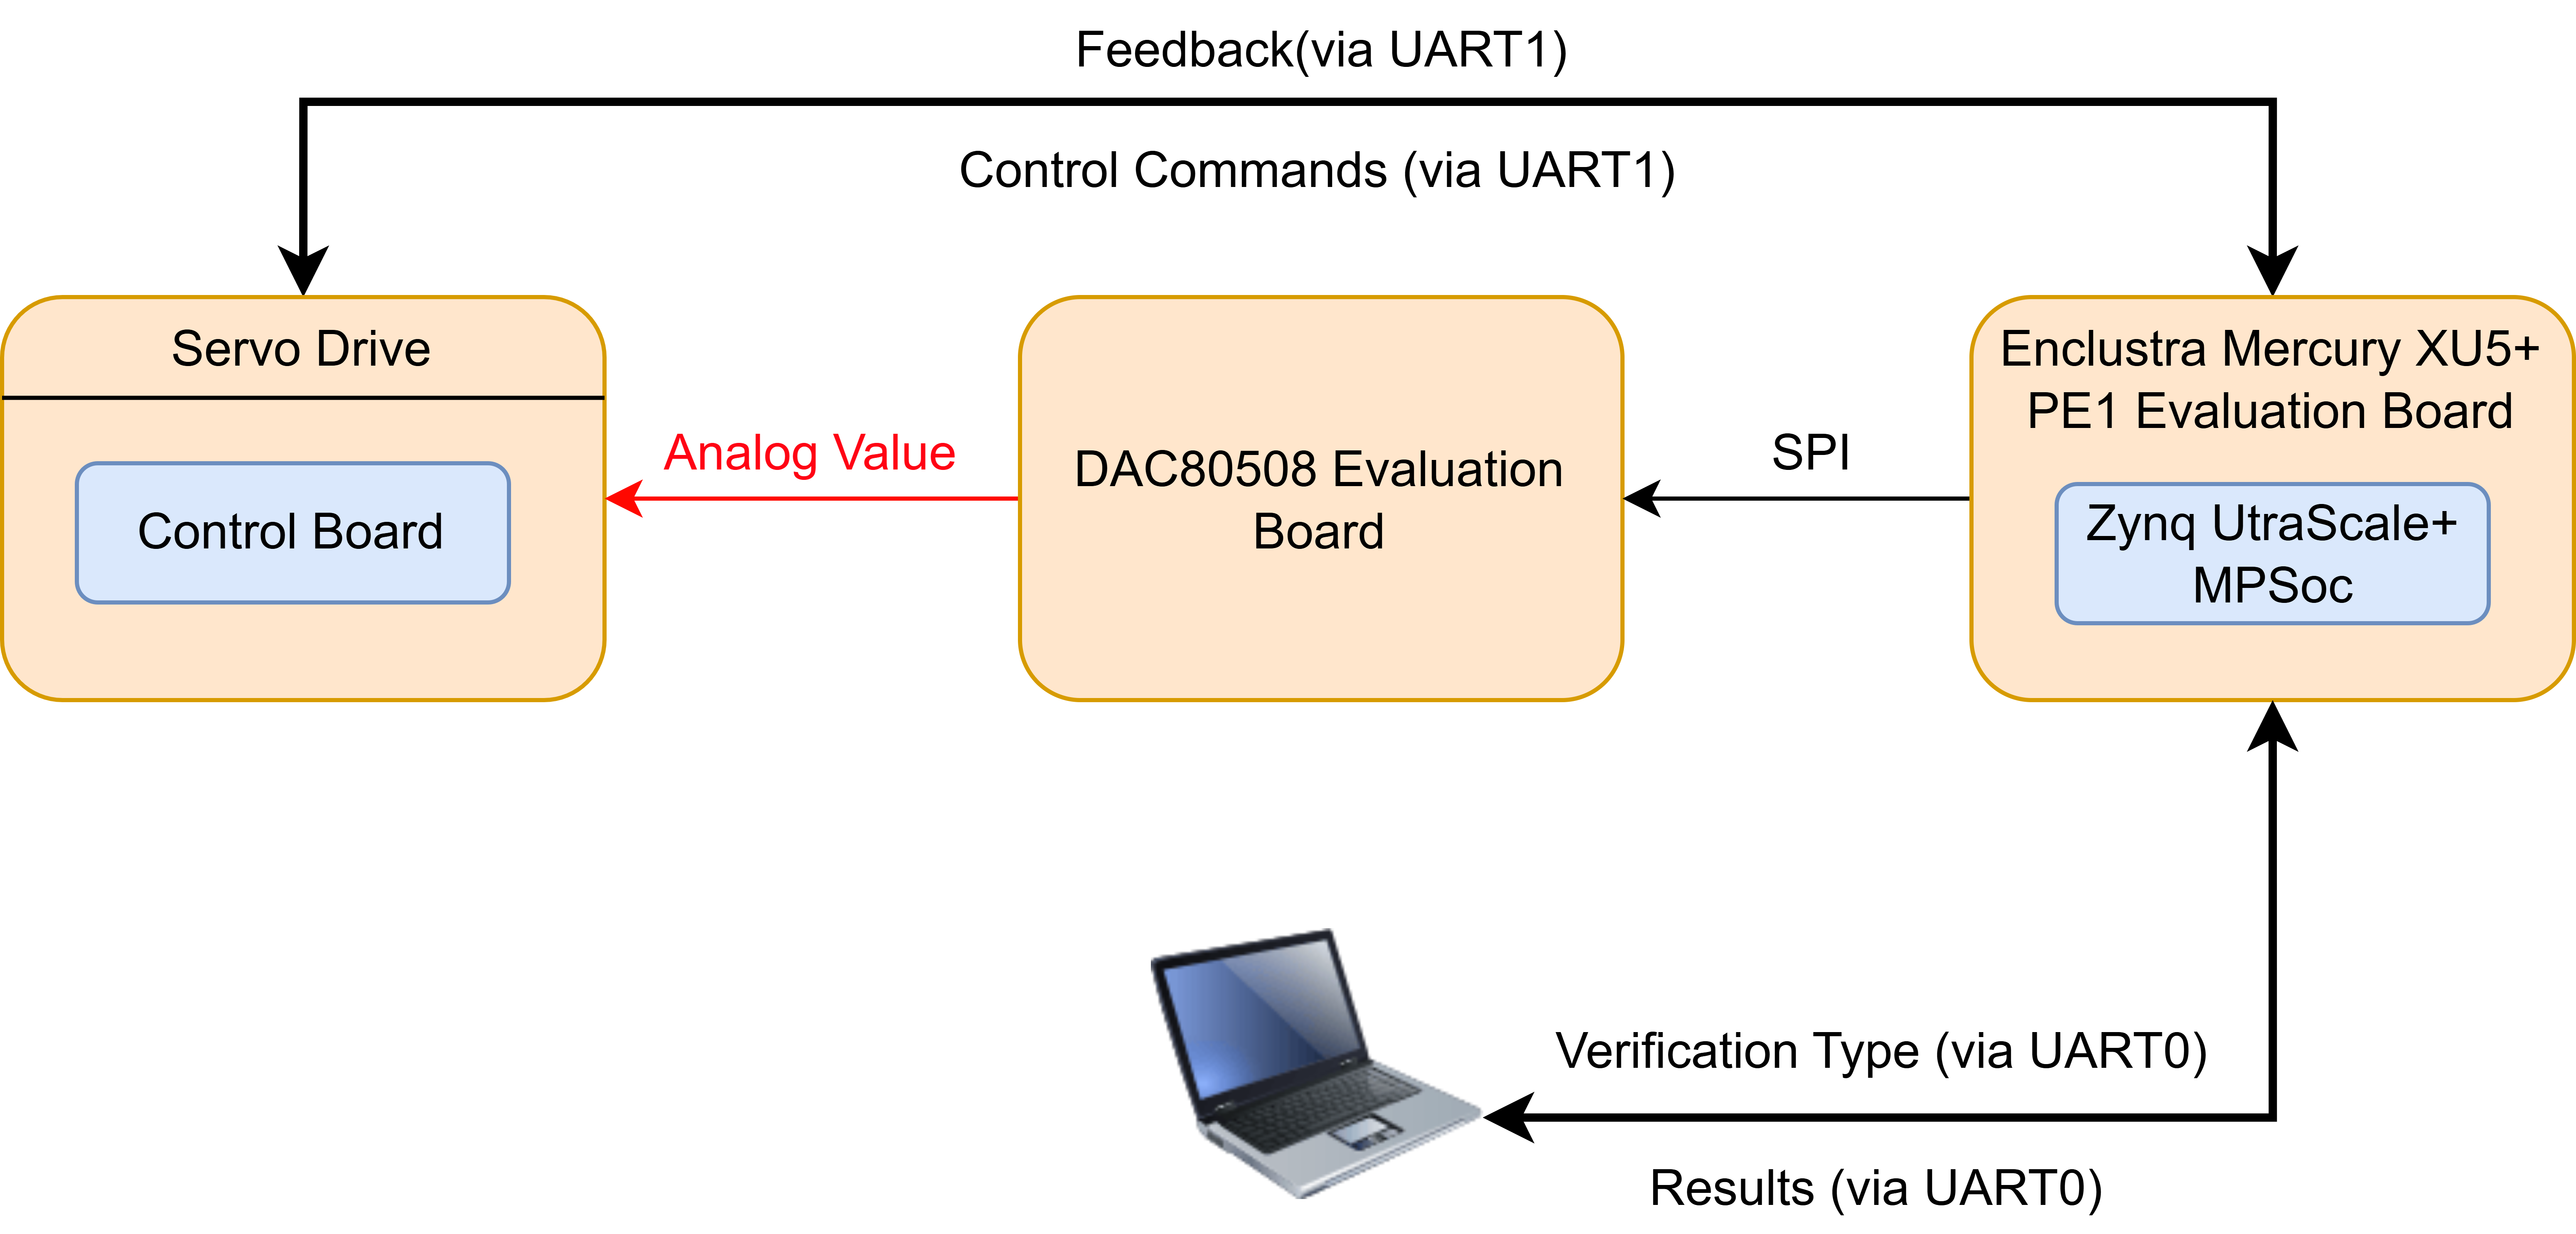
\includegraphics[width=1.00\textwidth, height=0.6\linewidth]{gfx/diagrams/BlockDiagram_PoC.png}
	\caption{Block Design of the \acs{FPGA} Verification Flatform \acs{PoC}}
	\label{fig:concept:PoC}
\end{figure}

This closed communication loop between the Verification \acs{SoC} and the Control Board enables detailed analysis of \acs{DUT} responses. By comparing the transmitted input data with the received feedback, the \acs{SoC} verifies whether the \acs{DUT} operates as intended under test conditions. This approach supports a systematic and reliable verification process, facilitating accurate testing of each \acs{FPGA} module and accommodating future design modifications. The block design of this \acs{PoC} demonstrates the feasibility of establishing an independent \acs{FPGA} verification setup capable of simulating real hardware interactions without requiring the complete motor control system.


\section{Related Work and Case studies in \acs{FPGA} and \acs{HIL} Verification}

The presented \acs{PoC} establishes a self-contained verification setup capable of generating analog signals, simulating motor feedback, and testing sensing and protection modules via a fully digital command-and-feedback loop. To contextualize this contribution within the broader research field, existing methods addressing similar verification challenges using \acs{FPGA}-based, \acs{HIL}, or \acs{FIL} techniques are reviewed. The review highlights key examples from power \acs{HIL}, \acs{FPGA}-in-the-Loop verification, and analog-interface emulation. Current gaps in the literature are identified, and it is demonstrated how this \acs{PoC} advances the field by providing low-power, closed-loop, and fully programmable verification for CurrentSense \acs{SPI} and protection logic.

\begin{enumerate}
	\item \textbf{"An \acs{FPGA}-in-the-Loop Approach for HDL Motor Controller Verification"} \cite{HDL_motorController_LiteratureSurvey}
	
	This paper presents the \acs{FIL} simulation methodology for verifying motor control systems that require concurrent simulation of both the control algorithm and the motor. Previous approaches that relied on prerecorded motor responses frequently yielded inaccurate results. In the \acs{FIL} approach, an \acs{FPGA} is programmed with the HDL design, and a simulated motor response is used to interact with the controller in a closed-loop configuration. This methodology was applied to implement, test, and validate both the Field-Oriented Control (FOC) algorithm and the Voltage-by-Frequency (V/f) control strategy for a Permanent Magnet Synchronous Machine (PMSM). The systems were designed in MATLAB Simulink and translated to VHDL using HDL Coder. \acs{FIL} simulation results closely matched software simulation results, indicating that prior discrepancies originated in the simulation method rather than the controller design. This approach may facilitate future controller switching for optimization or fault tolerance through Dynamic Partial Reconfiguration.
	
	\item \textbf{"\acs{FPGA}-based Real-Time Hardware-In-the-Loop Simulator of a Mini Solar Power Station"} \cite{Debreceni2014_MiniSolarHIL_LiteratureSurvey}
	
	The article describes the development of a real-time \acs{HIL} simulator that employs an \acs{FPGA} to model a miniature solar power station, specifically a solar panel-fed battery charger. The primary motivation for implementing \acs{HIL} is to enable safe, rapid testing of the digital controller unit (CU), thereby reducing the risks and costs of field testing and addressing parameter inaccuracies inherent in low-power laboratory models. The \acs{HIL} simulator replaces the high-power components of the system with computational models implemented in MATLAB/Simulink and running on the \acs{FPGA}. These simulated components interface with the control unit through physical connections, including analog and digital channels. The solar photovoltaic system model incorporates the effects of temperature and radiation by utilizing normalized characteristics stored in block RAMs as look-up tables for real-time computation. To generate the analog signals($\textit{u}_S, \textit{u}_A, \textit{i}_L$) required by the control unit's DSP, the simulator employs sigma-delta \acs{DAC}. The workflow leverages HDL synthesis from Simulink to reduce the need for manual code optimization.
	
	\item \textbf{"\acs{FPGA}-Based Real-Time Simulation of Nonlinear Permanent Magnet Synchronous Machines for Power Hardware-in-the-Loop Emulation Systems"} \cite{Schmitt2014_LiteratureSurvey}
	
	A real-time simulation system based on \acs{FPGA} technology is presented for modeling nonlinear Permanent Magnet Synchronous Machines in Power \acs{HIL} emulation systems. PHIL is designed to replace conventional, bulky motor-load testbeds with a flexible platform that can emulate various electric machines. The proposed machine model incorporates complex nonlinear phenomena, including magnetic anisotropy, iron saturation, and dynamic cross-coupling between the d- and q-axes. The primary contribution is a custom, high-performance signal-processing system that solves the machine’s differential equations at 1.5 MHz. Additionally, the model computes the counter-voltage required by the emulation converter, ensuring that the system accurately replicates the current slopes of an actual machine regardless of the inductance in the coupling network. The implementation employs fixed-point representation generated using MATLAB/Simulink and HDL Coder, achieving high accuracy with a relative error of less than 0.01\% in the current simulation compared to the floating-point model.

	\item \textbf{"\acs{FPGA}-synthesizable Filter Model Based Bitstream \acs{DAC} for Hardware-in-the-Loop Simulators"} \cite{Kokenyesi2016_BitstreamDAC_LiteratureSurvey}

	The article examines methods to enhance the analog output quality of \acs{FPGA}-based \acs{HIL} simulators, focusing on addressing the limited number of available \acs{FPGA} pins. Traditional Sigma-Delta (Σ-Δ) \acs{DAC} can be implemented on \acs{FPGA}s using a single pin per output, however, they require an analog low-pass filter, which restricts signal bandwidth and introduces phase delay. This limitation is particularly problematic for fast current control loops that frequently utilize triangular waveforms. The study proposes a novel Filter Model-Based \acs{DAC} architecture. The FMB \acs{DAC} incorporates a digital representation of the analog filter within the \acs{FPGA} to compensate for the low-pass filtering effect. A controller generates the bitstream by comparing the target input signal with the digital filter model's output. Experimental results demonstrate that, unlike conventional Σ-Δ DACs, the FMB \acs{DAC} accurately reproduces a 10 kHz triangular waveform with minimal phase delay and a significantly faster settling time. Additionally, it supports filter bandwidths up to 30 kHz. This performance improvement, however, comes at the cost of substantially increased \acs{FPGA} resource usage, requiring approximately four to five times more resources than a standard Σ-Δ \acs{DAC}.
		
\end{enumerate}

\subsection{\acs{PoC} Solutions to Identified Research Gaps}

\begin{itemize}
	\item \textbf{PHIL complexity vs verification scope}
	
	PHIL offers accurate power-level emulation, however it requires emulation converters, coupling networks, and precise management of converter dynamics. These requirements render PHIL expensive, complex, and potentially unsafe for routine module-level testing. Although existing studies demonstrate the advantages of PHIL, they also emphasize its logistical and cost challenges. \cite{Schmitt2014_LiteratureSurvey}
	
	This \acs{PoC} utilizes the Mercury XU5 System-on-Chip to generate both static and dynamic signals. A DAC80508 evaluation board converts these digital signals into analog currents or voltages, which are subsequently transmitted to the Control Board’s \acs{ADC}s. This configuration replicates the measurement behavior observed by the \acs{DUT} without requiring an emulation converter or power-level coupling network. It preserves essential sensing capabilities while significantly reducing complexity, cost, and safety risks compared to PHIL. Consequently, early-stage module testing becomes more feasible and secure.
	
	\item \textbf{Incomplete analog-chain verification in \acs{FIL}/\acs{HIL} workflows vs End-to-end verification that includes the analog acquisition chain}
	
	\acs{FIL} verifies HDL controller functionality and timing; however, it typically does not assess the analog sensing and acquisition chain, including \acs{DAC} fidelity, analog front-end filtering, \acs{ADC} timing, CurrentSense IC interaction, or \acs{SPI} readout. Consequently, sensor-level issues such as \acs{ADC} sampling shifts, CurrentSense \acs{SPI} timing problems, or analog filtering effects may remain undetected until full hardware integration \cite{HDL_motorController_LiteratureSurvey}.
	
	The \acs{PoC} stimulates the Control Board \acs{ADC} inputs with actual analog waveforms generated by the \acs{DAC} and evaluates the \acs{DUT} responses. This approach tests the entire measurement path, encompassing \acs{DAC} output fidelity, analog filtering and grounding, \acs{ADC} sampling, CurrentSense IC and \acs{SPI} behavior, and downstream \acs{FPGA} protection logic. It extends \acs{FIL}’s logic-level validation to include the complete sensor path.
	
	\item \textbf{Lack of targeted \acs{FPGA} module verification vs Automated command/feedback \acs{FPGA} module verification}
	
	Most existing research on \acs{HIL} and \acs{FIL} focuses on motor models, converter emulation, or controller parity. However, these studies do not directly address the \acs{FPGA} modules as the primary verification target\cite{Debreceni2014_MiniSolarHIL_LiteratureSurvey} .
	
	In the proposed \acs{PoC}, the \acs{SoC} transmits verification commands and parameters to the Control Board via UART1. The \acs{FPGA} on the Control Board executes the \acs{DUT} and returns the feedback. The \acs{SoC} subsequently verifies whether the \acs{DUT}'s feedback match the expected results and determines the test outcome. This automated command-and-feedback loop enables repeatable, parameterized test sequences and facilitates scalable regression-style verification for individual \acs{FPGA} modules. This approach represents an advancement over the manual \acs{HIL} setups described in previous research.

\end{itemize}


